\documentclass[12pt]{book}
%\usepackage[a4paper, margin=1.2in]{geometry}
\usepackage[a4paper,top=2cm, bottom=2cm, right=1.9cm, left=1.9cm]{geometry}

\usepackage[utf8]{inputenc}
\usepackage{amsmath,amssymb}
\usepackage[amsmath]{ntheorem}
\usepackage[bitstream-charter]{mathdesign}
\usepackage[dvipsnames]{xcolor}
\usepackage{listings}
\usepackage{courier}
\usepackage[hyphens]{url}
\usepackage{textcomp}
\usepackage{upquote}
\usepackage{graphicx}
\usepackage{tikz}
\usepackage{anyfontsize}
\usepackage[most]{tcolorbox}
\usepackage{setspace}
\usepackage[skip=10pt plus1pt, indent=0pt]{parskip}
\usepackage{booktabs}
\usepackage{svg}
\usepackage{mathtools}
\usepackage{annotate-equations}
\usepackage{subcaption}
\usepackage[leftcaption]{sidecap}
\usepackage{soul}
\usepackage{relsize}
\usepackage{wrapfig}
\usepackage{marginnote}
\usepackage{titlesec}
\usepackage{tabularx}
\usepackage{fancyhdr}
\usepackage{float}
\usepackage{enumitem}
\usepackage[colorlinks=true,linkcolor=black,anchorcolor=black,citecolor=black,filecolor=black,menucolor=black,runcolor=black,urlcolor=black,backref=page]{hyperref}
%\usepackage{emoji}

% Titlesec configuration
\titlespacing\section{0pt}{10pt plus 4pt minus 2pt}{10pt plus 4pt minus 2pt}
\titlespacing\subsection{0pt}{8pt plus 3pt minus 1pt}{8pt plus 3pt minus 1pt}

% Paragraph and spacing configuration
% \setstretch{1.25}
% \setlength{\parskip}{0pt}
% \setlength{\parindent}{0pt} % Disable indentation globally

% colors
\definecolor{drawgray}{HTML}{666666}
\definecolor{drawgray_l}{HTML}{F5F5F5}
\definecolor{drawblue}{HTML}{6C8EBF}
\definecolor{drawblue_l}{HTML}{DAE8FC}
\definecolor{drawgreen}{HTML}{82B366}
\definecolor{drawgreen_l}{HTML}{D5E8D4}
\definecolor{draworange}{HTML}{D79B00}
\definecolor{draworange_l}{HTML}{FFE6CC}
\definecolor{drawyellow}{HTML}{D6B656}
\definecolor{drawyellow_l}{HTML}{FFF2CC}
\definecolor{drawred}{HTML}{B85450}
\definecolor{drawred_l}{HTML}{EA6B66}
\definecolor{drawviolet}{HTML}{9673A6}
\definecolor{drawviolet_l}{HTML}{E1D5E7}
\definecolor{drawblackish}{HTML}{422222}

\definecolor{deepblue}{rgb}{0,0,0.5}
\definecolor{deepgreen}{rgb}{0,0.5,0}

\lstset{ 
  language=SQL,
  morekeywords={AFTER, INSTEAD, OF, REFERENCING, FOR, EACH, ROW, DECLARE, IF, TYPE, NEW, RETURNS, SELF, BEGIN, END, CONSTRUCTOR, UNDER, CONSTRUCTOR, STATIC, INSTANCE, RETURN, OVERRIDING, FINAL, NOT, INSTANTIABLE, UNNEST, MULTISET, ARRAY, COLLECT, METHOD, REF, MEMBER, FUNCTION, PROCEDURE, PRAGMA, RESTRICT_REFERENCES, WNDS, RNDS, TABLE, WITH, ASSIGNMENT, OPTIONS, SCOPE, NESTED, STORE, DEREF, VARRAY, OBJECT},
  framesep=1pt,
  xleftmargin=0pt,
  framexleftmargin=0pt,
  frame=tb,
  framerule=1pt,
  breaklines=true,
  commentstyle=\color{deepgreen},
  keywordstyle=\color{deepblue},
  showstringspaces=false,
  mathescape
}

\tcbset {
  base/.style={
    breakable,
    arc=0mm, 
    bottomtitle=0.5mm,
    boxrule=0mm,
    colbacktitle=drawblue_l, 
    colframe=drawblue,
    coltitle=black,
    fonttitle=\bfseries, 
    left=2.5mm,
    leftrule=1mm,
    right=3.5mm,
    title={#1},
    toptitle=0.75mm, 
  }
}

\newtcolorbox{supportbox}[1]{
  colframe=drawblue, 
  base={#1}
}

\definecolor{brandblue}{rgb}{0.34, 0.7, 1}
\newtcolorbox{mainbox}[1]{
colframe=brandblue, 
base={#1}
}

\newtcolorbox{subbox}[1]{
colframe=black!30!white,
base={#1}
}

\usepackage[style=0,ntheorem]{mdframed}
\mdfsetup{%
topline=false,
rightline=false,
bottomline=false,
linewidth=3pt,
innerleftmargin=15pt,
innerrightmargin=0pt,
skipabove=\baselineskip,
}
\newmdtheoremenv[linecolor=drawred]{definition}{Definition}[chapter]

\hypersetup{
    colorlinks=true,
    linkcolor=drawblackish,
    breaklinks=true,
    citecolor = drawblackish,
    urlcolor=drawblue,
}

% 1.15 spacing
\setstretch{1.15}

% Fancy header
\usepackage{fancyhdr}
\renewcommand{\chaptermark}[1]{\markboth{#1}{}}
\renewcommand{\sectionmark}[1]{\markright{#1}}
\fancyhead{} % clear all header fields
\fancyhead[LE]{{\color{black!40}\thepage}}
\fancyhead[RE]{\bfseries\normalfont {\color{black!40}\nouppercase{\rightmark}}}
\fancyhead[LO]{\bfseries\normalfont {\color{black!40}\nouppercase{Chapter \thechapter: \leftmark}}}
\fancyhead[RO]{{\color{black!40}\thepage}}

% Chapter title
\usepackage{titlesec, blindtext, color}
\definecolor{gray75}{gray}{0.75}
\newcommand{\hsp}{\hspace{20pt}}
\titleformat{\chapter}[hang]{\Huge\bfseries}{\selectfont \thechapter\hsp\textcolor{green}{|}\hsp}{0pt}{\Huge\bfseries}


\begin{document}

% \captionsetup[figure]{margin=1.5cm,font=small,labelfont={bf},name={Figure},labelsep=colon,textfont={it}}
% \captionsetup[table]{margin=1.5cm,font=small,labelfont={bf},name={Table},labelsep=colon,textfont={it}}

% diminuire il margine superiore della pagina mantenendo il margine inferiore
\newgeometry{top=2cm, bottom=2cm, right=2cm, left=2cm}

\begin{titlepage}
    \begin{center}
        
\includegraphics[width=0.6\textwidth]{img/uniba_logo.png}\\
          \vspace{1cm}
          % Dipartimento
          {\large Computer Science Department}\\
          \vspace{1cm}
          % Corso di laurea
          {\large Master Degree in Computer Science}\\
          \vspace{1cm}
          \hrule 
          \vspace{1.5cm}
          %{\large \textbf{LECTURE NOTES ON}}\\
          \vspace{0.5cm}
          % Materia
          {\large Practical Part of \textbf{Database Systems}}\\
          \vspace{1.5cm}
          % Titolo
          {\LARGE \textbf{Brightway}: Technical Documentation}
          \\ %% \textbf{Titolo della Tesi} 
          \vspace{1.2cm}

          \vfill
          
          \begin{tabularx}{\textwidth}{@{}Xr@{}}
              % Laureando e Relatori
              {\large Student:} & {\large Student ID:} \\  \\
              {\large \textbf{Mattia Curri} (\textit{\href{mailto:m.curri8@studenti.uniba.it}{m.curri8@studenti.uniba.it}})} & {\large \textbf{832437}} \\          \end{tabularx}    
          \vspace{1cm}
          \hrule
          \vspace{1cm}
          % Anno accademico in cui si è iscritti
          {\large ACADEMIC YEAR \textbf{2024{-}2025}}
    \end{center}
\end{titlepage}
\restoregeometry

\tableofcontents
\newpage
\pagestyle{fancy}

\chapter{Requirements}

\begin{figure}[H]
    \centering
    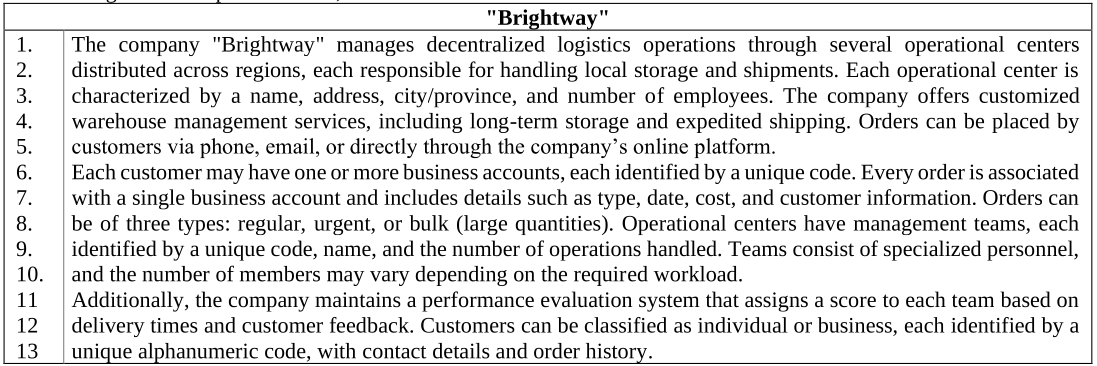
\includegraphics[width=1.0\textwidth]{img/requirements.png}
\end{figure}
\chapter{Conceptual Design}

\section{Requirements Analysis}



\section{Reorganize sentences for specific concepts}


\begin{tcolorbox}[title=General Phrases]
We want to create a database that manages decentralized logistics operations through several operational centers, storing information about orders, teams, and customers. The company offers customized warehouse management services, including long-term storage and expedited shipping.
\end{tcolorbox}

\begin{tcolorbox}[title=Phrases related to Operational Centers]
Operational centers are distributed across regions, each responsible for handling local storage and shipments.  

For each operational center, we will hold name, address, city/province, and number of employees.  

Operational centers have management teams.
\end{tcolorbox}

\begin{tcolorbox}[title=Phrases related to Orders]
Orders can be placed by customers via phone, email, or online.  

For each order, we will hold type, date, cost, and customer information.  

Every order is associated with a single business account.  

Orders can be of three types: regular, urgent, or bulk (large quantities).
\end{tcolorbox}

\begin{tcolorbox}[title=Phrases related to Business Accounts]
Each business account will be identified by a unique code.  

Each customer may have one or more business accounts.  

Every order is associated with a single business account.
\end{tcolorbox}

\begin{tcolorbox}[title=Phrases related to Teams]
For each team, we will identify them via a unique code, and we will hold name and number of orders handled.  

Teams consist of employees, and the number of employees may vary depending on the required workload.  

The company maintains a performance evaluation system that assigns a score to each team based on delivery times and customer feedback.
\end{tcolorbox}

\begin{tcolorbox}[title=Phrases related to Customers]
Each customer may have one or more business accounts.  

Customers can be classified as individual or business, each identified by a unique alphanumeric code, with contact details and order history.
\end{tcolorbox}

\begin{tcolorbox}[title=Phrases related to Employees]
Teams consist of employees, and the number of employees may vary depending on the required workload.
\end{tcolorbox}

\section{Level of abstraction}
For \textbf{customer information}, we consider \textit{name}, \textit{surname}, and \textit{date of birth} for individual customers, and \textit{company name} and \textit{address} for business customers, where the address consists of \textit{street}, \textit{civic number}, \textit{city}, \textit{province}, \textit{region}, and \textit{state}.  

For \textbf{contact details}, we consider \textit{phone number} and \textit{email}.  

\textbf{Specialized personnel} is replaced by \textit{employees}.  

\textbf{Number of members} is replaced by \textit{number of employees}.  

\textbf{Number of operations} is replaced by \textit{number of orders}.

\section{Glossary of terms}
\begin{table}[h!]
    \resizebox{\textwidth}{!}{
    \begin{tabular}{|c|p{5cm}|p{3cm}|p{3cm}|}
    \hline
    \textbf{Term} & \textbf{Description} & \textbf{Synonyms} & \textbf{Connections} \\
    \hline
    Operational Center & Decentralized locations handling local storage and shipments. Characterized by name, address, city/province, and number of employees. & / & Team \\
    \hline
    Order & Requests for services or goods from customers, identified by type (regular, urgent, or bulk). Includes type, date, cost, and customer details. & Operation & Customer, Business Account, Team \\
    \hline
    Business Account & Accounts tied to customers, containing unique codes and details like orders and customer type (individual or business). & Account & Customer, Order \\
    \hline
    Team & Groups of employees linked to an operational center, evaluated on delivery times and customer feedback. & Management Team & Operational Center, Order, Employee \\
    \hline
    Customer & Individuals or businesses placing orders. Identified by unique alphanumeric codes, contact details, and order history. & Individual, Business & Order, Business Account \\
    \hline
    Employee & Specialized personnel working in teams and handling orders. & Specialized Personnel & Team \\
    \hline
    \end{tabular}
    }
    \end{table}

\subsection{Skeleton ER Schema}
\begin{figure}[H]
    \centering
    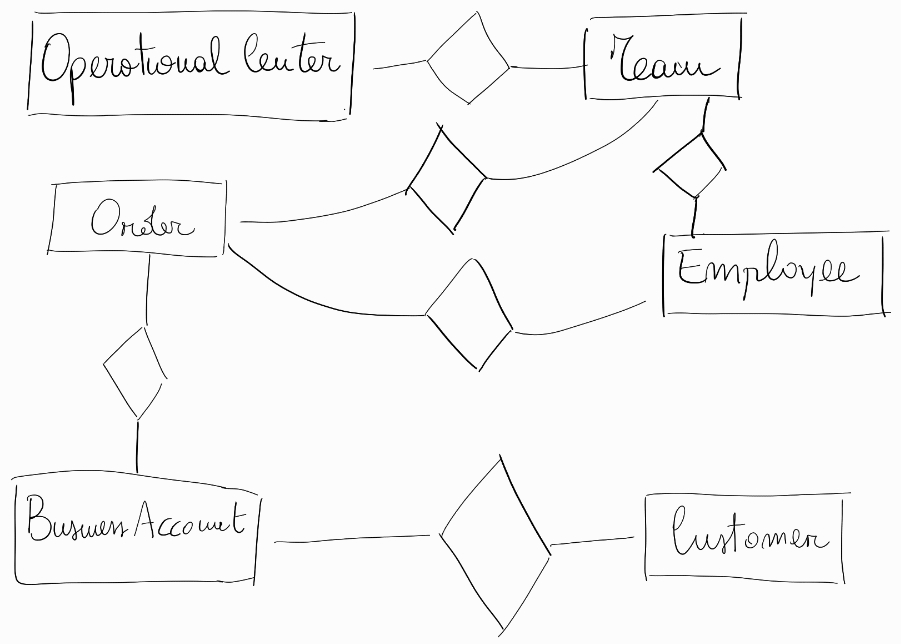
\includegraphics[width=0.8\textwidth]{img/skeleton.png}
\end{figure}

\subsection{Final ER Schema}
\begin{figure}[H]
    \centering
    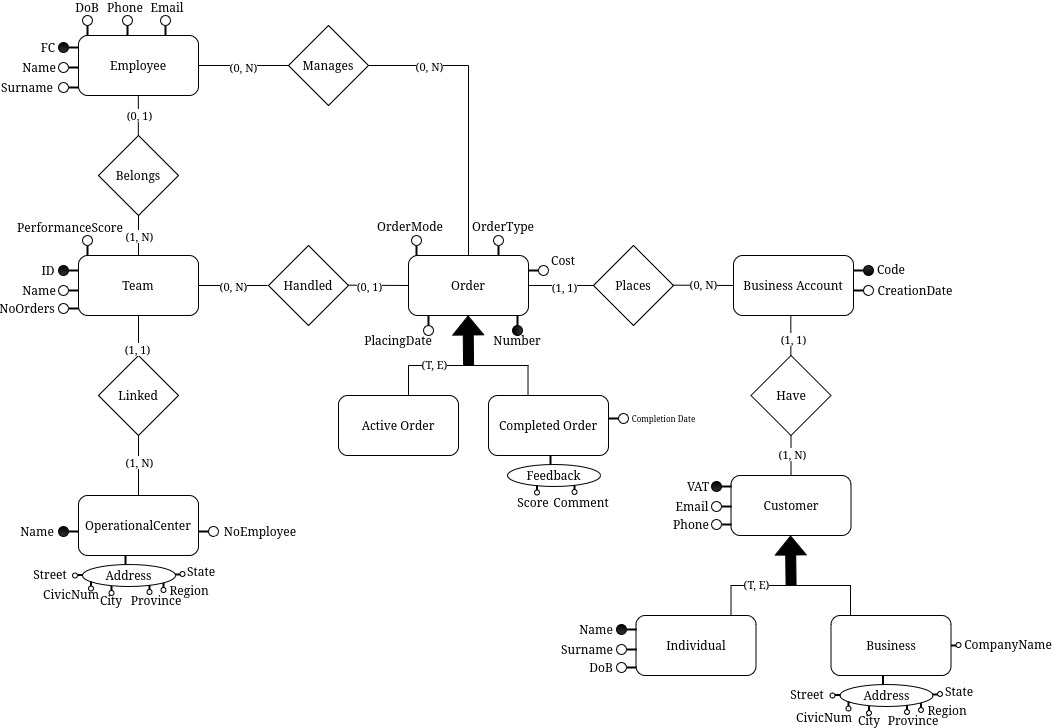
\includegraphics[width=0.8\textwidth]{img/ER.jpg}
\end{figure}

\begin{itemize}[label=-]
    \item There are three redundancies: \texttt{NoOrders} and \texttt{PerformanceScore} in \texttt{Team} and \texttt{NoEmployee} in \texttt{Operational Center}, that will be evaluated later.
    \item There are two generalizations for \texttt{Order} and \texttt{Customer}, that will be evaluated later.
\end{itemize}

\section{Business Rules}
\begin{itemize}
    \item Employees linked to an order must be in the same team that handle the order.
    \item Number of employees is the sum of all employees in a team.
    \item Number of orders is the sum of all orders handled by a team.
    \item Completion date cannot be before placing date.
    \item PerformanceScore is computed as the mean of all feedbacks.
    \item A team has a maximum of 8 members.
    \item OrderType must be of three types: regular, urgent, or bulk.
    \item OrderMode must be of three types: phone, email, or online.
    \item Feedback of CompletedOrder must be between 1 and 5.
    \item A feedback cannot be given before the order is completed.
    \item A team must be assigned before an order is completed.
    \item A team cannot be changed after an order is completed.
    \item Employees of a completed order cannot be changed.
    \item An order can be deleted only if there are not information for the business account or for the feedback computation.
\end{itemize}



\chapter{Logical Design}
\section{Volumes Table}
We will consider a span of a month to evaluate the volumes of the entities.

\begin{table}[h!]
    \resizebox{\textwidth}{!}{
    \begin{tabular}{|l|c|p{14cm}|c|}
    \hline
    \textbf{Concept} & \textbf{Type} & \textbf{Computation} & \textbf{Final Volume} \\
    \hline
    Operational Center & E & 15 (assuming 10 team per \texttt{Operational Center}) & 15 \\
    \hline
    Linked To & R & 150 (same as \texttt{Team}) & 150 \\
    \hline
    Team & E & 150 (\textit{given}) & 150 \\
    \hline
    Handled By & R & 45000 (same as (assigned) \texttt{Order}) & 45000 \\
    \hline
    Order & E & $300 \; \text{op/m} \cdot 150 \cdot 12 + 100 \; \text{not assigned}$ & 45100 \\
    \hline
    Belongs To & R & $150 \; \texttt{Team} \cdot 6.4 \; \text{current \texttt{Employee}}$ & 960 \\
    \hline
    Employee & E & $80\% \; \text{of} \; (150 \cdot 8) + 140 \; \text{past \texttt{Employee}}$ & 1100 \\
    \hline
    Manages & R & $45000 \cdot 3 \; \text{(assuming 3 \texttt{Employee} working on an \texttt{Order})}$ & 135000 \\
    \hline
    Places & R & $45100 \; \text{(same as \texttt{Order})}$ & 45100 \\
    \hline
    Business Account & E & $\dfrac{45100 \; \texttt{Order}}{1.5 \; \text{\texttt{Order}/month}}$ & 30000 \\
    \hline
    Have & R & $30000 \; \text{(same as \texttt{Business Account})}$ & 30000 \\
    \hline
    Customer & E & $\dfrac{30000 \; \texttt{Business Account}}{1.5 \; \text{\texttt{Business Account}/\texttt{Customer}}}$ & 20000 \\
    \hline
    Active Order & E & $20\% \; \text{of} \; 45000 + 100 \; \text{not assigned}$ & 9100 \\
    \hline
    Completed Order & E & $80\% \; \text{of} \; 45000$ & 36000 \\
    \hline
    Individual & E & $90\% \; \text{of \texttt{Customer}}$ & 18000 \\
    \hline
    Business & E & $10\% \; \text{of \texttt{Customer}}$ & 2000 \\
    \hline
    \end{tabular}
    }
\end{table}
    

\section{Operations Analysis}
\begin{table}[h!]
    \centering
    \caption{Operations frequency analysis}
    \begin{tabular}{|l|c|c|}
    \hline
    \textbf{Operation} & \textbf{Type} & \textbf{Frequency} \\
    \hline
    Operation 1 & I & 10/day \\
    \hline
    Operation 2 & I & 1000/day \\
    \hline
    Operation 3 & I & 500/day \\
    \hline
    Operation 4 & I & 200/day \\
    \hline
    Operation 5 & I & 20/day \\
    \hline
    \end{tabular}
    \end{table}
    
    In the next section, we will double count the cost of writing operations.
    
    \subsection*{Operation 1: Register a new customer}
    
    \begin{table}[h!]
    \centering
    \caption{Access analysis for registering a new customer}
    \begin{tabular}{|l|c|c|c|}
    \hline
    \textbf{Concept} & \textbf{Type} & \textbf{No. Access} & \textbf{Access Type} \\
    \hline
    Customer         & E & 1 & W \\
    \hline
    Have             & R & 1 & W \\
    \hline
    Business Account & E & 1 & W \\
    \hline
    \end{tabular}
    \end{table}
    
    \textbf{Operation cost}: $6 \; \text{accesses} \cdot 10 \; \text{days} = 60 \; \text{accesses/day}$
    
    \subsection*{Operation 2: Add a new order}
    
    \begin{table}[h!]
    \centering
    \caption{Access analysis for adding a new order}
    \begin{tabular}{|l|c|c|c|}
    \hline
    \textbf{Concept} & \textbf{Type} & \textbf{No. Access} & \textbf{Access Type} \\
    \hline
    Order   & E & 1 & W \\
    \hline
    Places  & R & 1 & W \\
    \hline
    \end{tabular}
    \end{table}
    
    \textbf{Operation cost}: $4 \; \text{accesses} \cdot 1000 \; \text{days} = 4000 \; \text{accesses/day}$
    
    \subsection*{Operation 3: Assign an order to a management team}
    
    Access \textit{without} redundancy \texttt{Team.NoOperations}:
    
    \begin{table}[h!]
    \centering
    \caption{Access analysis for assigning order to team (without redundancy)}
    \begin{tabular}{|l|c|c|c|}
    \hline
    \textbf{Concept} & \textbf{Type} & \textbf{No. Access} & \textbf{Access Type} \\
    \hline
    Handled By & R & 1 & W \\
    \hline
    Manages    & R & 3 & W \\
    \hline
    \end{tabular}
    \end{table}
    
    Access \textit{with} redundancy \texttt{Team.NoOperations}:
    
    \begin{table}[h!]
    \centering
    \caption{Access analysis for assigning order to team (with redundancy)}
    \begin{tabular}{|l|c|c|c|}
    \hline
    \textbf{Concept} & \textbf{Type} & \textbf{No. Access} & \textbf{Access Type} \\
    \hline
    Handled By & R & 1 & W \\
    \hline
    Team       & E & 1 & R \\
    \hline
    Team       & E & 1 & W \\
    \hline
    Manages    & R & 3 & W \\
    \hline
    \end{tabular}
    \end{table}
    
    \textbf{Operation cost} (\textit{without redundancy}): $8 \; \text{accesses} \cdot 500 \; \text{days} = 4000 \; \text{accesses/day}$ 

    \textbf{Operation cost} (\textit{with redundancy}): $11 \; \text{accesses} \cdot 500 \; \text{days} = 5500 \; \text{accesses/day}$
    
    \subsection*{Operation 4A: View the total number of operations handled by a specific team}
    
    Access \textit{with} redundancy \texttt{Team.NoOperations}:
    
    \begin{table}[h!]
    \centering
    \caption{Access analysis for viewing team operations (with redundancy)}
    \begin{tabular}{|l|c|c|c|}
    \hline
    \textbf{Concept} & \textbf{Type} & \textbf{No. Access} & \textbf{Access Type} \\
    \hline
    Team    & E & 1 & R \\
    \hline
    \end{tabular}
    \end{table}
    
    Access \textit{without} redundancy \texttt{Team.NoOperations}:
    
    \begin{table}[h!]
    \centering
    \caption{Access analysis for viewing team operations (without redundancy)}
    \begin{tabular}{|l|c|c|c|}
    \hline
    \textbf{Concept}    & \textbf{Type} & \textbf{No. Access} & \textbf{Access Type} \\
    \hline
    Handled By & R & 300 & R \\
    \hline
    \end{tabular}
    \end{table}
    
    \textbf{Operation cost} (\textit{with redundancy}): $1 \; \text{access} \cdot 200 \; \text{days} = 200 \; \text{accesses/day}$  

    \textbf{Operation cost} (\textit{without redundancy}): $300 \; \text{accesses} \cdot 200 \; \text{days} = 60000 \; \text{accesses/day}$
    \subsection*{Operation 4B: Show the total cost of the orders handled by a specific team}
    
    TODO
    
    \subsection*{Operation 5: Print a list of teams sorted by their performance score}
    
    Access \textit{with} redundancy \texttt{Team.PerformanceScore}:
    
    \begin{table}[h!]
    \centering
    \caption{Access analysis for sorting teams by performance (with redundancy)}
    \begin{tabular}{|l|c|c|c|}
    \hline
    \textbf{Concept} & \textbf{Type} & \textbf{No. Access} & \textbf{Access Type} \\
    \hline
    Team    & E & 150 & R \\
    \hline
    \end{tabular}
    \end{table}
    
    Access \textit{without} redundancy \texttt{Team.PerformanceScore}:
    
    \begin{table}[h!]
    \centering
    \caption{Access analysis for sorting teams by performance (without redundancy)}
    \begin{tabular}{|l|c|c|c|}
    \hline
    \textbf{Concept} & \textbf{Type} & \textbf{No. Access} & \textbf{Access Type} \\
    \hline
    Team       & E & 150    & R \\
    \hline
    Handled By & R & 45000  & R \\
    \hline
    Order      & E & 45000  & R \\
    \hline
    \end{tabular}
    \end{table}
    
    \textbf{Operation cost} (\textit{with redundancy}): $150 \; \text{accesses} \cdot 20 \; \text{days} = 3000 \; \text{accesses/day}$  

    \textbf{Operation cost} (\textit{without redundancy}): $90150 \; \text{accesses} \cdot 20 \; \text{days} = 1803000 \; \text{accesses/day}$
    

\section{Redundancy Analyisis}
\begin{itemize}[label=-]
\item \texttt{OperationalCenter.NoEmployees}: given that there are no operations that involve this attribute, so we decide to \textbf{eliminate} the redundancy.
\item \texttt{Team.NoOperations}: with the redundancy, we have 4200 accesses combining both Op. (3) and (4); on the other hand, without the redundancy, we have 65700 accesses. In the end, we decide to \textbf{maintain} the redundancy.
\item \texttt{Team.PerformanceScore}: with the redundancy, we have 3000 accesses on Op. (5); on the other hand, without the redundancy, we have 1803000 accesses. In the end, we decide to \textbf{maintain} the redundancy.
\end{itemize}

\section{Partitioning and Merging}
\begin{itemize}[label=-]
    \item Merging \texttt{Actual Order} and \texttt{Completed Order} into \texttt{Order}: given the fact that there are not operations that require to distinguish between the two entities, we can \textbf{merge} them into a single entity.
    \item Merging \texttt{Individual} and \texttt{Business} into \texttt{Customer}: given the fact that there are not operations that require to distinguish between the two entities, we can \textbf{merge} them into a single entity.
\end{itemize}

\subsection{Restructured Schema}
INSERIRE SCHEMA UML


\chapter{Implementation}

\subsection*{Types definition}
\begin{lstlisting}
CREATE OR REPLACE TYPE AddressTY AS OBJECT (
    street VARCHAR2(50),
    civicNum NUMBER,
    city VARCHAR2(50),
    province VARCHAR2(50),
    region VARCHAR2(50),
    state VARCHAR2(50)
);
\end{lstlisting}

\begin{lstlisting}
CREATE OR REPLACE TYPE OperationalCenterTY AS OBJECT (
    name VARCHAR2(50),
    address AddressTY
);
\end{lstlisting}

\begin{lstlisting}
CREATE OR REPLACE TYPE TeamTY AS OBJECT (
    ID VARCHAR2(32),
    name VARCHAR2(20),
    numOrder NUMBER,
    performanceScore NUMBER(4, 2),
    operationalCenter ref OperationalCenterTY
);
\end{lstlisting}

\begin{lstlisting}
CREATE OR REPLACE TYPE EmployeeTY AS OBJECT (
    FC VARCHAR2(16),
    name VARCHAR2(20),
    surname VARCHAR2(20),
    dob DATE,
    phone VARCHAR2(14),
    email VARCHAR2(50),
    team ref TeamTY
);
\end{lstlisting}

\begin{lstlisting}    
CREATE OR REPLACE TYPE FeedbackTY AS OBJECT (
    score NUMBER(1),
    commentF VARCHAR2(1000)
);
\end{lstlisting}

\begin{lstlisting}    
CREATE OR REPLACE TYPE CustomerTY AS OBJECT (
    VAT VARCHAR2(11),
    phone VARCHAR2(14),
    email VARCHAR2(50),
    type VARCHAR2(10),
    name VARCHAR2(20),
    surname VARCHAR2(20),
    dob DATE,
    companyName VARCHAR2(50),
    address AddressTY
) NOT FINAL;
\end{lstlisting}

\begin{lstlisting}    
CREATE OR REPLACE TYPE BusinessAccountTY AS OBJECT (
    CODE VARCHAR2(32),
    creationDate DATE,
    customer ref CustomerTY
);
\end{lstlisting}

\begin{lstlisting}
CREATE OR REPLACE TYPE EmployeeVA AS VARRAY(8) OF REF EmployeeTY;
\end{lstlisting}

\begin{lstlisting}    
CREATE OR REPLACE TYPE OrderTY AS OBJECT (
    ID VARCHAR2(32),
    placingDate DATE,
    orderMode VARCHAR2(6),
    orderType VARCHAR2(7),
    cost NUMBER(10, 2),
    businessAccount ref BusinessAccountTY,
    team ref TeamTY,
    employees EmployeeVA,
    completionDate DATE,
    feedback FeedbackTY
);
\end{lstlisting}

\subsection*{Table definition}
\begin{lstlisting}
CREATE TABLE OperationalCenterTB OF OperationalCenterTY (
    name PRIMARY KEY,
    address NOT NULL
); 
\end{lstlisting}

\begin{lstlisting}
CREATE TABLE TeamTB OF TeamTY (
    ID PRIMARY KEY,
    name NOT NULL,
    numOrder check (numOrder >= 0),
    performanceScore check (performanceScore between 1 and 5),
    operationalCenter NOT NULL
);
\end{lstlisting}

\begin{lstlisting}
CREATE TABLE EmployeeTB OF EmployeeTY (
    FC PRIMARY KEY CHECK (LENGTH(FC) = 16),
    name NOT NULL,
    surname NOT NULL,
    dob NOT NULL,
    phone NOT NULL,
    email NOT NULL
);
\end{lstlisting}

\begin{lstlisting}
CREATE TABLE CustomerTB OF CustomerTY (
    VAT PRIMARY KEY CHECK (LENGTH(VAT) = 11),
    phone NOT NULL,
    email NOT NULL,
    type NOT NULL CHECK (type IN ('individual', 'business'))
);
\end{lstlisting}

\begin{lstlisting}
CREATE TABLE BusinessAccountTB OF BusinessAccountTY (
    CODE DEFAULT RAWTOHEX(SYS_GUID()) PRIMARY KEY,
    creationDate NOT NULL,
    customer NOT NULL
);
\end{lstlisting}

\begin{lstlisting}
CREATE TABLE OrderTB OF OrderTY (
    ID DEFAULT RAWTOHEX(SYS_GUID()) PRIMARY KEY,
    placingDate NOT NULL,
    orderMode NOT NULL CHECK (orderMode IN ('online', 'phone', 'email')),
    orderType NOT NULL CHECK (orderType IN ('regular', 'urgent', 'bulk')),
    cost NOT NULL CHECK (cost > 0),
    businessAccount NOT NULL,

    check (placingDate <= completionDate),
    check (feedback.score between 1 and 5)
);
\end{lstlisting}


\chapter{Trigger Implementation}

\section{Triggers}

\subsection*{CheckOrderInsertOrUpdate}
This trigger enforces logical constraints on orders:
\begin{lstlisting}[language=SQL]
CREATE OR REPLACE TRIGGER CheckOrderInsertOrUpdate
    % ...existing code...
END;
/
\end{lstlisting}

\subsection*{CheckCustomerType}
Enforces that "individual" customers cannot have business data and vice versa:
\begin{lstlisting}[language=SQL]
CREATE OR REPLACE TRIGGER CheckCustomerType
    % ...existing code...
END;
/
\end{lstlisting}

\subsection*{UpdateNumOrders}
Keeps each team's numOrder up-to-date when orders are inserted, updated, or deleted:
\begin{lstlisting}[language=SQL]
CREATE OR REPLACE TRIGGER UpdateNumOrders
    % ...existing code...
END;
/
\end{lstlisting}

\subsection*{CheckTeamInsertInitialization}
Initializes numOrder and performanceScore when inserting a new team:
\begin{lstlisting}[language=SQL]
CREATE OR REPLACE TRIGGER CheckTeamInsertInitialization
    % ...existing code...
END;
/
\end{lstlisting}

\subsection*{CheckNumEmployeeInTeam}
Ensures a team cannot exceed 8 employees:
\begin{lstlisting}[language=SQL]
CREATE OR REPLACE TRIGGER CheckNumEmployeeInTeam
    % ...existing code...
END;
/
\end{lstlisting}

\subsection*{ComputePerformanceScore}
Recalculates a team's average feedback score whenever a new order or feedback is added or updated:
\begin{lstlisting}[language=SQL]
CREATE OR REPLACE TRIGGER ComputePerformanceScore
    % ...existing code...
END;
/
\end{lstlisting}

\subsection*{AddAccount}
Automatically creates a business account for every new customer:
\begin{lstlisting}[language=SQL]
CREATE OR REPLACE TRIGGER AddAccount
    % ...existing code...
END;
/
\end{lstlisting}

\subsection*{DeleteTeamAfterOperationalCenter}
Deletes teams that lose their operational center reference upon an operational center's deletion:
\begin{lstlisting}[language=SQL]
CREATE OR REPLACE TRIGGER DeleteTeamAfterOperationalCenter
    % ...existing code...
END;
/
\end{lstlisting}

\subsection*{UpdateEmployeeAfterTeam}
Sets an employee's team reference to NULL if the team is deleted, and unassigned orders if they're not completed:
\begin{lstlisting}[language=SQL]
CREATE OR REPLACE TRIGGER UpdateEmployeeAfterTeam
    % ...existing code...
END;
/
\end{lstlisting}

\subsection*{DeleteAccountAfterCustomer}
Deletes business accounts that become orphaned when their customer is removed:
\begin{lstlisting}[language=SQL]
CREATE OR REPLACE TRIGGER DeleteAccountAfterCustomer
    % ...existing code...
END;
/
\end{lstlisting}

\subsection*{DeleteOrdersAfterTeam}
Removes orders that have lost their team and business account references:
\begin{lstlisting}[language=SQL]
CREATE OR REPLACE TRIGGER DeleteOrdersAfterTeam
    % ...existing code...
END;
/
\end{lstlisting}

\subsection*{DeleteOrdersAfterAccount}
Deletes orders that have lost their related business account, under certain conditions:
\begin{lstlisting}[language=SQL]
CREATE OR REPLACE TRIGGER DeleteOrdersAfterAccount
    % ...existing code...
END;
/
\end{lstlisting}

\subsection*{PreventOrderDeletion}
Prevents order deletion unless it has lost all references or is uncompleted with no account:
\begin{lstlisting}[language=SQL]
CREATE OR REPLACE TRIGGER PreventOrderDeletion
    % ...existing code...
END;
/
\end{lstlisting}

\subsection*{EmptyEmployeeListAfterTeamUpdate}
Clears the employee list if a team reference changes:
\begin{lstlisting}[language=SQL]
CREATE OR REPLACE TRIGGER EmptyEmployeeListAfterTeamUpdate
    % ...existing code...
END;
/
\end{lstlisting}


% ...existing code...

\chapter{Functions Implementation}

\section{Operations Implementation}

\subsection{Operation 1: registerCustomer}
Registers a new customer with optional business or individual data.
\begin{lstlisting}[language=SQL]
CREATE OR REPLACE PROCEDURE registerCustomer(
    VAT IN VARCHAR2,
    phone IN VARCHAR2,
    email IN VARCHAR2,
    type IN VARCHAR2,
    name IN VARCHAR2,
    surname IN VARCHAR2,
    dob IN DATE,
    companyName IN VARCHAR2,
    address IN AddressTY
) AS
    customer CustomerTY;
BEGIN
    % ...existing code...
END;
/
\end{lstlisting}

\subsection{Operation 2: addOrder}
Adds a new order by referencing a business account and optional employees.
\begin{lstlisting}[language=SQL]
CREATE OR REPLACE PROCEDURE addOrder(
    ID IN VARCHAR2,
    placingDate IN DATE,
    orderMode IN VARCHAR2,
    orderType IN VARCHAR2,
    cost IN NUMBER,
    businessAccountName IN VARCHAR2,
    employees IN EmployeeVA DEFAULT NULL
) AS
    % ...existing code...
END;
/
\end{lstlisting}

\subsection{Operation 3: assignOrderToTeam}
Assigns an order to a specific team.
\begin{lstlisting}[language=SQL]
CREATE OR REPLACE PROCEDURE assignOrderToTeam(
    orderID IN VARCHAR2,
    teamID IN VARCHAR2
) AS
    % ...existing code...
END;
/
\end{lstlisting}

\subsection{Operation 4A: totalNumOrder}
Returns the total number of orders handled by a given team.
\begin{lstlisting}[language=SQL]
CREATE OR REPLACE FUNCTION totalNumOrder(
    teamID IN VARCHAR2
) RETURN NUMBER AS
    % ...existing code...
END;
/
\end{lstlisting}

\subsection{Operation 4B: totalOrderCost}
Calculates the total cost of all orders for a team.
\begin{lstlisting}[language=SQL]
CREATE OR REPLACE FUNCTION totalOrderCost(
    teamID IN VARCHAR2
) RETURN NUMBER AS
    % ...existing code...
END;
/
\end{lstlisting}

\subsection{Operation 5: printTeamsByPerformanceScore}
Prints teams sorted by performance score in descending order.
\begin{lstlisting}[language=SQL]
CREATE OR REPLACE PROCEDURE printTeamsByPerformanceScore AS
BEGIN
    % ...existing code...
END;
/
\end{lstlisting}


\input{sections/6_physical_design}

\input{sections/7_web_app.tex}



\end{document}
